\chapter{Minimum Broadcast Time}\label{sec:mbt}

Broadcasting is the information dissemination process in a communication network.
The Minimum Broadcast Time (MBT) problem is identified by a set of communication devices (nodes), among which some selected ones acts as an originators of a signal.
The number of originators is at least one, and we refer them as \emph{sources}.
The task is to spread a signal from the sources to the remaining nodes along the communication links defined by edges $E$ in a shortest possible time.
The continuous time is divided into discrete time steps.
The communication among the nodes must fulfill the following rules:
\begin{enumerate}
\item Each transmission takes place between two adjacent nodes
\item Each transmission requires one time step
\item Each node can participate in at most one transmission per one time step
\end{enumerate}

This communication protocol appears in various practical applications such as communication among computer processors and telephone networks.
In satellite networks, even though the communication is wireless, signals have to cover large distances, 
and so the information is sent from one satellite to one of its neighbours at a time.
The MBT problem was studied in the context of an existing Chinese BeiDou Global Navigation Satellite System~\cite{chu17}.

\section{Network Model and Definitions}

The communication network is determined by a graph $G=(V,E)$ and a subset $S\subseteq V$ of sources.

\begin{definition}
The broadcast time $\tau(G,S)$ of $S\subseteq V$ in $G$ is defined as the smallest integer $t\geq 0$
for which there exists a sequence $V_0\subseteq\dots\subseteq V_t$ of node sets and a function $\pi:V\setminus S\mapsto V$, satisfying:
\begin{enumerate}
\item $V_0=S$ and $V_t=V$,
\item for all $v\in V\setminus S, \left\{v,\pi(v)\right\}\in E$,
\item for all $k=1,\dots t$ and all $v\in V_k$, $\pi(v)\in V_{k-1}$, and
\item for all $u,v\in V_k\setminus V_{k-1}$, $\pi(u)=\pi(v)$ only if $u=v$.
\end{enumerate}
\end{definition}

The \emph{broadcast center} of a graph is the set of all nodes having the smallest broadcast times ,i.e., $\arg\min\left\{\tau(G,\{v\}):v\in V\right\}$.

Formally, the optimization MEB problem is defined as follows:
\begin{problem}\label{mbt:opt}
Given $G=(V,E)$ and $S\subseteq V$, find $\tau(G,S)$. 
\end{problem}

In the literature, authors often consider the decision version, because some of the theoretical results depend on a given time limit.
\begin{problem}\label{mbt:dec}
Given $G=(V,E)$, $S\subseteq V$,  and a time limit $t$, does $\tau(G,S)\leq t$ hold? 
\end{problem}
%\section{Problem Definition}

%\section{Broadcast Graphs}

\section{Computational Complexity}

MBT has been thoroughly studied from the perspective of computation complexity and approximability, particularly in the early 90'.
ITS NP-completeness or belonging to P was shown for various graph classes and values of time limit $t$.

It has been shown that the problem is NP-complete for arbitrary graphs in \cite{garey79} and few years later, 
this result was obtained for arbitrary graphs with deadline $t=4$ and a single source by reduction from \textsc{3D Matching}~\cite{slater81}. 
The same work also contains a $\mathcal{O}(n)$ algorithm for determining broadcast time of a tree with a single source. 
As a by-product, this algorithm determines the broadcast center of the input tree.

These results are improved and extended in~\cite{jansen93}, where the authors exploit the properties of NP-complete problem \textsc{Planar 3-SAT}.
First, they prove that \textsc{Planar 3,4-SAT} is NP-complete, and subsequently use this property to show that MBT is NP-complete for:
\begin{itemize}
\item bipartite planar graphs, deadline $t=2$ and maximum degree at most 3,
\item split graphs with deadline $t=2$,
\item chordal graphs with a single source, 
\item planar graphs with single source and maximum degree at most 3, 
\item bipartite planar graphs with maximum degree at most 3 and a single source,
\item grid graphs with deadline $t=2$ and maximum degree at most 3,
\item grid graphs with a single source, and
\item complete grid graphs with deadline $t=2$. 
\end{itemize}
The question whether MBT is NP complete for split graphs with a single source is stated as open.
Another complexity result proving that MBT remains NP-complete for 3-regular planar graphs with constant deadline $t\geq 2$ 
is given in \cite{middendorf93} by reduction from \textsc{Exactly-one-in-three-3SAT}.

The complexity results above typically exploit sophisticated reductions.
We provide a very simple and straightforward proof of NP-completeness of MEB for time limit at most $t=4$.
There are many restrictions on SAT that preserve NP-completeness.
We concentrate on the variant of 3SAT with the property that each variable is restricted to appear at most three times, and each literal at most twice. 
This problem is known as 3-3-SAT, and its NP-completeness proof can be found in~\cite{papadimitriou94}. 
Note that in this particular version of 3SAT, it can no longer be assumed that each clause consists of exactly 3 literals.
Further, the assumption about at most two occurrences of a literal is automatic, 
because formula $\varphi$ that contains a variable $x$ that appears only as a positive or only as a negative literal can trivially be transformed into $\varphi'$ that does not contain $x$ at all, 
such that $\varphi$ is satisfiable if and only if $\varphi'$ is satisfiable.
\begin{lemma}
Let $\varphi$ be an instance of \textsc{3-3-SAT}, and let $G=(V,E)$ and $S\subseteq V'$ be an instance of MEB constructed from $\varphi$. 
Then, $\varphi$ is satisfiable if and only if $\tau(G,S)\leq 4$.
\end{lemma}
\begin{proof}\label{prop:mbtnpc}
An instance of Problem \ref{prob:dec} is constructed from an instance $\varphi(x_1,\dots,x_n)$ of 3-3-SAT as follows.
For each variable $x_i$ in $\varphi$, we construct a gadget comprising six nodes $x_i$, $\bar{x}_i$, $u_i$, $v_i$, $w_i$ and a source $s_i$.
The first two nodes represent possible literals associated with the variable $x_i$.
The gadget further contains five edges $\{s_i,u_i\}$, $\{u_i,x_i\}$, $\{u_i,\bar{x}_i\}$, $\{u_i,v_i\}$, and $\{v_i,w_i\}$.
For each clause $c_j$, there is a node $c_j$ and whenever the clause $c_j$ contains a literal $x_i$ ($\bar{x}_i$), there is an edge $\{c,x_i\}$ ($\{c,\bar{x}_i\}$).
We therefore have clause nodes of degree at most 3, because $\varphi$ is in 3-CNF.
Nodes representing literals are connected to at most two clause nodes, which is implied by the restriction imposed on $\varphi$.
In a solution $T$ to the constructed instance (highlighted as blue)  $\arg\min\limits_{v\in\{x,\bar{x}\}}\{t_{u_x,v}\}$ represents the assignment of truth value to the variable $x$.
The presence of an arc entering a clause node $c$ in $T$ indicates that a truth value of certain variable caused satisfaction of clause $c$.
The auxiliary path $(u_x,v_x,w_x)$ ensures that the clause satisfaction is modeled correctly.
As $t_{u_x,v_x}\leq 3$, one of $t_{u_x,x}$ and $t_{u_x,\bar{x}}$ must be 4, 
and thereby the arc that would incorrectly indicate satisfaction of a clause that is not satisfied by the selected truth assignment would have cost 5, which is not allowed.
It is possible to have and arc outgoing from a clause node of cost 4, but the second endpoint is always a node representing some literal $y$, but the arc $(u_y,y)$ is already a part of $T$.
\end{proof}
\begin{proposition}

\end{proposition}
For illustrating the construction in the proof of Prop.~\ref{prop:mbtnpc}, consider the following instance of \textsc{3-3-SAT}
\begin{equation}
\varphi=(x_1\vee x_2\vee x_3)\wedge(\bar{x}_1\vee x_4)\wedge(x_2\vee \bar{x}_3 \vee\bar{x}_4)\wedge(\bar{x}_1\vee \bar{x}_3)\wedge \bar{x}_2 
\label{eq:phi}
\end{equation}
reducing to the instance of Problem \ref{mbt:dec} depicted in Fig. \ref{fig:mbtnpc}.
\begin{figure}
\centering
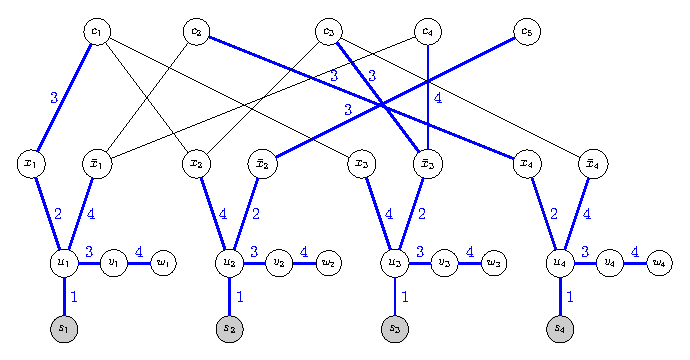
\includegraphics{figurer/mbtnpc.eps}
\caption{Reduction}
\label{fig:mbtnpc}
\end{figure}




\section{Solution Techniques}
